\documentclass[5pt]{article}
\usepackage{multicol,multirow}
\usepackage{graphicx} % Required for inserting images
\usepackage[margin=0.75cm]{geometry}
\usepackage{xcolor}
\usepackage{amsmath}
\usepackage{mathtools}
\usepackage{relsize}

\usepackage[english]{babel}
\newtheorem{theorem}{Theorem}

\usepackage{empheq}
\usepackage{amsfonts}

\usepackage{tkz-euclide}
\usepackage{tikz}

\definecolor{LightGray}{gray}{0.9}

\usepackage{minted}

\DeclarePairedDelimiter\abs{\lvert}{\rvert}%
\DeclarePairedDelimiter\norm{\lVert}{\rVert}%

\makeatletter
\let\oldabs\abs
\def\abs{\@ifstar{\oldabs}{\oldabs*}}

\newcommand{\tr}[3]{
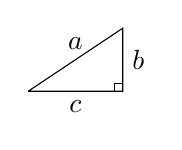
\begin{tikzpicture}[scale=0.40]
    \coordinate [] (A) at (-1.5cm,-1.cm);
    \coordinate [] (C) at (1.5cm,-1.0cm);
    \coordinate [] (B) at (1.5cm,1.0cm);
    \draw (A) -- node[above] {$a$} (B) -- node[right] {$b$} (C) -- node[below] {$c$} (A);
    \draw (1.25cm,-1.0cm) rectangle (1.5cm,-0.75cm);
\end{tikzpicture}
}


\begin{document}


\begin{center}
     \Large{\textbf{Python Programming}}\\
     \small{Class: COSC 1800}\hfill\small{\textcopyright Maximilien Notz \the\year{}}
     \noindent\rule{20.2cm}{0.4pt}
\end{center}


\begin{multicols}{2}
\setcounter{secnumdepth}{0}

\subsection{General Reminder}
\begin{tabular}{ll}
    random.randint(x,y)     & Generate a random integer between \textbf{x}\\
                            & and \textbf{y}(import random).\\
    type(var)               & Returns the type of var.\\
    type(n, b, d,)          & Dynamicaly create a class named \textbf{n}.\\
                            & This class inerits all classes in \textbf{b} (tuple).\\
                            & \textbf{d} is a dictionary containing attributes\\
                            & and member method.\\
\end{tabular}
\begin{minted}[bgcolor=LightGray]{Python}
    if conditon_1:
        # code if conditon_1 is true
    elif conditon_2:
        # code if conditon_2 is true
    else:
        # code
\end{minted}


\subsection{Operators}
\begin{tabular}{|ll|ll|}
    \hline
    +   & addition & //  & div\\
    -   & substraction & and & logical and\\
    *   & multiplication & or  & logical or\\
    /   & division & not & logical not\\
    \%  & modulo & a in b  & is  \textbf{a} in  \textbf{b}?\\
    **  & power & a==b & is  \textbf{a} equal to  \textbf{b}? \\
    \hline
\end{tabular}



\subsection{Error Handling}

\subsection{Object Oriented Programing(OOP)}

%%%%%%%%%%%%%%%%%%%%
%% CODE %%%%%%%%%%%%
%%%%%%%%%%%%%%%%%%%%

\end{multicols}
\end{document}